\documentclass[10pt,conference]{IEEEtran}
%\documentclass[a4paper,12pt]{article}
%\usepackage{algpseudocode}
\usepackage{cite,latexsym,times,epsf,amsmath,amssymb,amsfonts,graphicx}
\usepackage{epstopdf}
\usepackage{graphicx}
\usepackage{subfigure}
\usepackage{multirow}
\usepackage{algorithmic}
\usepackage{algorithm}
\usepackage{amsmath}
\usepackage{verbatim}
\usepackage{booktabs}
\usepackage{authblk}
\usepackage{bm}
\renewcommand{\algorithmicrequire}{\textbf{Input:}}
\renewcommand{\algorithmicensure}{\textbf{Output:}}
\renewcommand{\baselinestretch}{0.915}
%\renewcommand{\algorithmicforall}{\textbf{Foreach}}
%\renewcommand{\algorithmicendfor}{\textbf{}}


\begin{document}
\title{WhiteCell: Leveraging Scant White Space Resource in Dense Area}
\author{Pengfei Cui}
\author{Dinesh Rajan}
\author{Joseph Camp}
\affil{Department of Electrical Engineering, Southern Methodist University}
%\documentclass[10pt]{article}

%\usepackage{xkvltxp}


\maketitle


\begin{abstract}

%While many metropolitan areas sought to deploy city-wide WiFi networks, the densest urban areas were not
%able to broadly leverage the technology for large-scale Internet access.  Ultimately, the small 
%spatial separation required for effective 802.11 links in these areas resulted in prohibitively large up-front 
%costs.  

The FCC has reapportioned spectrum from TV white spaces for the purposes of large-scale Internet 
connectivity via wireless topologies of all kinds. 
The far greater range of these lower carrier frequencies are especially critical in dense areas, where 
high levels of aggregation could adapt the mobility of users.
However, the restriction of white space in dense area limits the available number of white space channels 
in dense areas. 
Thus, leveraging the range of spectrum across user mobility becoms a critical issue for the deployment of 
data networks with WiFi and white space bands. 
% Work
In this paper, we measure the spectrum utility in typical environment of the Dallas-Fort Worth metropolitan. 
We formulate the heterogeneous wireless network with both WiFi and white space bands as a queuing system. 
Further, we propose a measurement-driven resource allocation algorithm, Greedy Server-side Replace (GSR).
In particular, we study the white space and WiFi bands with in-field spectrum utility measurements, revealing 
the power consumption required for an area with channels in multiple bands. In doing so, we find that 
networks with white space bands in dense areas reduce the power consumption by up to FIXME 
% In sparse area, the power consumption is the most


\end{abstract}

\section{Introduction}
\label{sec:introduction}

%  Multiband background
The FCC has approved the use of broadband services in the white spaces of 
UHF TV bands, which were formerly exclusively licensed to television broadcasters.
These white space bands are now available for unlicensed public use, enabling the
deployment of wireless access networks. These white space bands operate in available 
channels from 54-806 MHz, having a far greater propagation range than WiFi bands for 
similar transmission power~\cite{balanis2012antenna}. 
% Improve existing cells
Thus, white space bands could greatly complement the existing WiFi wireless network with 
a large area. The users in the propagation range of the access point with white space radios 
has the options to associate with either the WiFi channel of its cell or the white space 
channel.



% Multi-user diersity
The users in multiple locations under the coverage of both the WiFi and white space have {\it user 
diversity}. The term user diversity represents the same frequency band at the same time can offer 
different transmission qualities to different users due to their difference in transceiver design, 
geographic location, etc.
% Explain the spectral diversity temporal diversity
The user diversity comes from two types of diversity gains. One is the temporal diversity which 
is caused by the environment variation. Another is the spectral diversity which represents the 
transmission conditions varies across channels. 
In some moderate number of users, the sum capacity of the fading channel is greater than 
the sum capacity of a nonfading channel. In the fading channels, the sum capacity of users 
increase with the number of users in the system~\cite{viswanath2002opportunistic,gan2014multiple}. 


% White space limited resource
%Moreover, the number of available white space channels are restricted by FCC. In sparse rural area,
%there are more free channels in white space. Inversely, few available channels are located in dense 
%populated area. The question {\it how limited white space resource befinet the access of the users 
%in these diversity scenarios?}

Previous work studied the multi user setting with a single channel~\cite{tan2010distributed}. Spectral diversity 
is isolated for a single user in~\cite{shu2009throughput}. In~\cite{liu2013stay}, multi-user dynamic channel access is 
proposed jointly consider the temporal and spectral diversity in a multichannel model. However, 
none of these works address the channel association problem in multiband scenario.

The larger propagation range of white space channels adapt channel association of users located 
in large area through time division. When the users distributed in a large area, the temporal 
diversity and spectral diversity become the key issues of white space applications.
Previous work~\cite{pcuiwinmee} studied the white space application in access network deployment 
with spectral diversity. However, these works fails to leverage the white space frequency in 
multi-user diversity in both spectral and temporal scenarios.

% Extreme cases and the middle of number of channels
In sparse rural areas, plenty of white space channels are able to deploy new white space network. However, 
in dense area, few white space channels are available for new network deployment, such as none white 
space channel is available in New York downtown~\cite{googlespectrum}. The carrier have to use WiFi 
channels to deploy wireless networks in the dense area without any available white space channel. 
Other than these two extreme cases, most areas of major cities in the United States have one to eight 
white space channels~\cite{googlespectrum}. Exploiting these limited white space resource to improve 
the WiFi network in dense area is a perspective option for the dense areas.

% Power saving, extreme cases
The white space frequencies offer more wireless capacity and convenience of access across large 
area. When the traffic demands of the users are relatively low, a single white space channels satisfy 
all the user. Then, the WiFi radios could be turned off for saving power. On the other side, 
when the users have high traffic demand, all the radios, WiFi and white space, have to be operated to serve the users. 
However, traffic demands generally come across somewhere between these extremes.
Thus, the question comes out,a{\it in what degree the white space help to reduce the power consumptions of 
an existing WiFi mesh?} 

% Traffic Demand
In this work, we study channel schedule in a multi-user multiband setting, where users are not 
fully backlogged, traffic demand follow a certain arrival process. We focus on the effect of channel 
schedule of each user between the WiFi or white space band. 

% On demand consideration

% Paper contributions
In particular, the main contributions of our work are as follows:
\begin{itemize}
\item We perform long-term in-field measurements in neighborhoods, campus, downtown business building, 
and urban business buildings. Through the measurements, we estimate the achieved channel capacity in 
these area.
\item We formulate the channel resource allocation problem as a queuing system. Based on previous works, we 
propose the response time estimation methods of multiple scenarios for the heterogeneous network.
\item We develop a Greedy Server-side Replace algorithm to allocate the channel capacity for the users with minimum 
power consumption.
\item We perform measurement-driven simulation to analyze various scenarios of channel resource and users distribution. 
Our results shows that the white space bands reduce the power consumption in typical city environment by FIXME.
\end{itemize}

The rest of the paper 

\section{System, Assumptions and Problem Formulation}
\label{sec:problemformulation}

% Background and problem model
\subsection{System and Assumptions}
\label{subsec:model}
% Background
% Multiband variation
Wireless propagation refers to the signal loss characteristics when wireless signals 
are transmitted through the wireless medium. The strength of the received signal depends on 
both the line-of-sight path (or lack thereof) and multiple other paths that result from reflection, 
diffraction, and scattering from obstacles~\cite{andersen1995propagation}. The widely-used Friis
equation characterizes the received signal power $P_r$ in terms of transmit power $P_t$, transmitter 
gain $G_t$, receiver gain $G_r$, wavelength $\lambda$ of the carrier frequency, distance $R$ from 
transmitter to receiver, and path loss exponent $n$ according to~\cite{friis}:
\begin{equation}
\label{eq:friis}
P_r=P_t+G_t+G_r+10n \log_{10}\left( \frac{\lambda}{4\pi R}\right)
\end{equation}
Here, $n$ varies according to the aforementioned environmental 
factors with a value ranging from two to five in typical outdoor 
settings~\cite{rappaport}.
% White spcae is good out resource to improve the service of Wifi cell
The propagation range of low frequency white space channels is many times larger than high frequency WiFi channels, for instance, 
450 MHz channels has more than 12 times the propagation range of 5 GHz channels via Friis model. Thus, with a 
single white space access point is possible to serve an area up to hundred times of a WiFi access point. 
The large propagation of white space channels can potentially be applied for the reduction of network deployment 
cost~\cite{pcuiwinmee}, the adaptation of vehicular dynamic access~\cite{chen2011feasibility}, and improvement 
of network capacity~\cite{bahl2009white}.
However, previous works that focus on the application of many white space channel resources or point to point 
communication requiring a small amount of white space resource fail to investigate heterogeneous networks 
with limited white space resources.

\begin{table*}[hpt]
\centering % centering table 
\begin{tabular}{|l|c|c|c|c|c|c|c|} % 
\hline %\hline % inserting double-line 
City & New York & Log Angeles & San Francisco & Seattle & Houston & Austin & Dallas \\
\hline %\hline % inserting double-line 
White space channels & 0 & 0 & 2 & 7 & 3 & 1& 3 \\
\hline %\hline % inserting double-line 
\end{tabular}    
\caption{Number of White Space Channels in Major Cities} % title name of the table 
\label{tab:whitespacechannel}    
\vspace{-0.3in}
\end{table*}    

In wireless network design, 
more wireless channel resources bring more flexibility and better performance.
White space frequency is the new opportunity for wireless networks. 
However, the FCC restricts the number of white space channels in most dense urban areas 
to protect existing television broadcasts. 
The minimum number of white space channels in some major cities of the U.S are listed in 
Table~\ref{tab:whitespacechannel}~\cite{googlespectrum}.
In New York and Los Angeles, some districts have zero white space channel available.
Part of Austin has only one white space channel available in dense urban areas.
Most of the other cities in the table have 2 to 7 white space channels.
Thus, it is unfeasible to implement white space wireless networks 
with limited resources in these dense urban areas.
% WiFi cells exist
Moreover, most of the dense areas already have deployed wireless networks. 
Our proposed wireless system leverages the existing infrastructure, adding additional
frequency efficiency and lower energy usage.

% Power saving
\begin{figure}
\vspace{-0.0in}
\centering
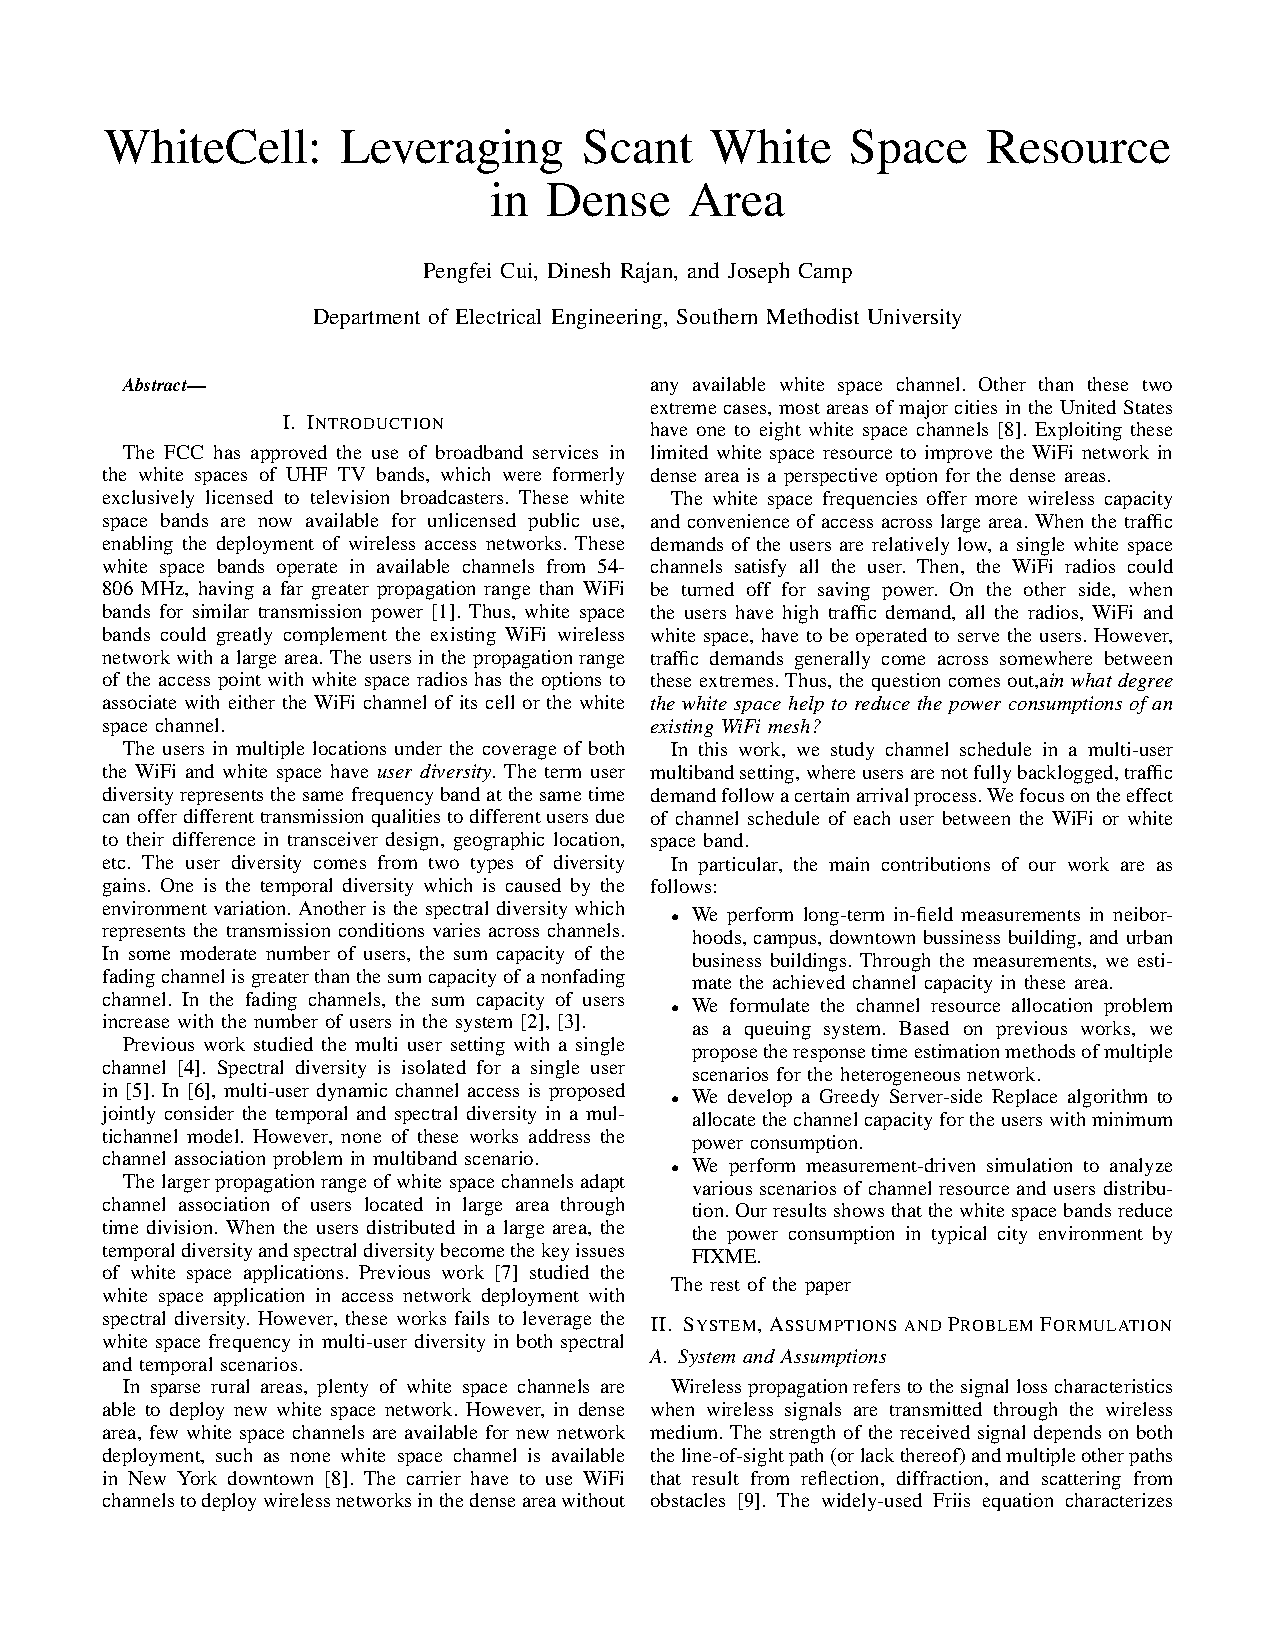
\includegraphics[width=84mm]{figures/whitecell}
\vspace{-0.1in}
\caption{Heterogeneous WhiteCell Structure}
\label{fig:systemmodel}
\vspace{-0.3in}
\end{figure}

% Give the model and assumption
% B channel; N user; M AP;
Here, we introduce a heterogeneous network structure named WhiteCell with existing wireless 
cells and reusing the central access point with few white space radios as shown in 
Fig.~\ref{fig:systemmodel}.
The cells are deployed via high frequency cellular or WiFi, which we refer to as WiFi cells 
later on.
Given a mesh wireless system with $M$ cells and access points and $N$ users.
The white space radios are installed on the access point in the central cell.
The large propagate white space channels in the system cover all the existing cells while 
each cell has its own wireless resource previously assigned other than the white space resource.
Thus, the users of each cell have access to the white space channels and the assigned single cell  
channel. 
The reuse of WiFi and cellular channels has been discussed in plenty of previous works and it is 
out of our scope.
$F_w$ is the white space radios installed on the central cell access point.
The white space channels are able to be split for multiple cells access point in the system.
We assume the capacity in an environment that is clean of all the radios is $C$. 
There is enough buffer to store the traffic coming from the users on each access point.
The traffic aggregated at the access point could be transferred through the single cell 
frequency resources or the shared white space resources.
The traffic is served in a first-in-first-out (FIFO) scheduling strategy.
In this structure, the traffic of each cell could be transferred by $F_w+1$ channels.
The one is the single cell wireless channel and the others are the white space channels.
We assume the users in the same mesh cell are in a single interference domain. 
Considering the limited number of white space channels in dense areas and considering spatial reuse 
of white space makes the problem considerably more challenging, it remains an interesting 
direction for future research. 

Instead of assuming the wireless channels are on-off~\cite{bodas2012low} or have equal capacity, 
we apply a measurement driven estimation to get the achieved channel capacity. The capacity of the 
channel between the access points and each user is noted as a matrix in Eq.~\ref{eq:usercapacity}
\begin{equation}
\label{eq:usercapacity}
H_{i,j}^f(t)= G(\zeta,t),i \in M, j\in N, f \in (F_M+F_w) 
\end{equation} 
$\zeta$ represents the in-field measured historical data and dynamic sensing information.
A context-aware method is applied to estimate the $j$th user capacity $H_{i,j}^f(t)$ to an access point 
$i$ on channel $f$. The users in a single cell have the same channel status. We assume the channel 
capacity is flat during a certain time slot. The switching time is negligible in the system.
The calculation of achieved channel capacity is introduced in~\ref{subsec:experimentsetup}. 
The traffic demand of a user obey Poisson process, with the vector noted as 
$\bm{D(t)} = [D_1(t),D_2(t),...D_N(t)]$ and the sum rate $D(t) = \sum\limits_{i=1}^N D_i(t)$. 
The rate $D(t)$ is the aggregate rate of data generated from all users. 

% tolerance time, energy model
During a time slot, the unscheduled radios remain in sleep mode to save energy. We also ignore 
the sleeping energy as well as the amount of energy spent on channel or radio switching. An operating 
radio will cost equal standby power per unit time. Previous human factor work~\cite{niida2010user} 
shows users have a certain patience for response. 
The tolerance time of users varies across the traffic type, such as text information, 
voice and video. To simply the problem, we assume an average value for tolerance response time $W$ 
of all the users in the system. 
With the same number of traffic demand, more channel capacity offers more data rate which reduce 
the response time.
Thus, the longer the tolerance time required by the users, the more channel capacity resource is 
required.

\subsection{Problem Formulation}
\label{subsec:problem}

We formulate the heterogeneous wireless network system introduced in~\ref{subsec:model} as a 
discrete-time queuing system shown in Fig.~\ref{fig:flowconfig}. 
The channels are represented as servers in the queuing model. 
Table.~\ref{tab:notation} summarizes the notation used in this work. 
In the system, there are $F_w$ white space radios and $M$ cells. 
$F_M$ represents the single cell resource radios allocated to $M$ cells. 
Multiple cells may share the same single cell resource, but there is no overlap of their service areas.
Thus, the queuing system has $M$ queues of the cells and $F_M+F_w$ servers in total connecting 
by time-varying channels $H^*(M,F_M+F_w)$.

\begin{table}[htbp]
\begin{center}% used the environment to augment the vertical space
% between the caption and the table
\begin{tabular}{l l p{10cm} }
\toprule
$t$ & Time slot\\
$N$ & Set of users\\
$M$ & Set of WiFi cells\\
$H_{ij}^f$ & Measurement based Capacity between AP i and user j on channel f\\
$F_{m}$ & WiFi Channels in the cells\\
$F_{w}$ & Set of White Space Channels\\
$A(t)$ & User access channel schedule\\
$C$ & Clean Radio Capacity\\
$D$ & User Demand\\
$R$ & Operating Radio\\
$\zeta$ & In-Field Measurements\\
$W$ & User Tolerance time window \\
$\mu$ & Channel capacity assigned for a cell \\
$P_s$ & Standby Power Consumption \\
$P_t$ & Transmission Power Consumption \\
%$R_{i}$ & $\triangleq$ & Revenue at store $i$\\
%$i$ & $\triangleq$ & index value for store locations\\
%${T}_{c}$ & $\triangleq$ & A very long description of this specific variable and is needed in the research and looks good when wrapped and aligned to the left.\\
%$TC$ & $\triangleq$ & Total overall cost(\$)\\  
%\multicolumn{3}{c}{}\\
%\multicolumn{3}{c}{\underline{Decision Variables}}\\
%\multicolumn{3}{c}{}\\
%$y_f$ & $=$ & \(\left\{\begin{array}{rl}
%1,  & \text{if Supplier located at site $f$ is open} \\
%0,  & \text{otherwise} \end{array} \right.\)\\
\bottomrule
\end{tabular}
\end{center}
\caption{Table of Notations}
\label{tab:notation}
\vspace{-0.3in}
\end{table}


\begin{figure}
\vspace{-0.0in}
\centering
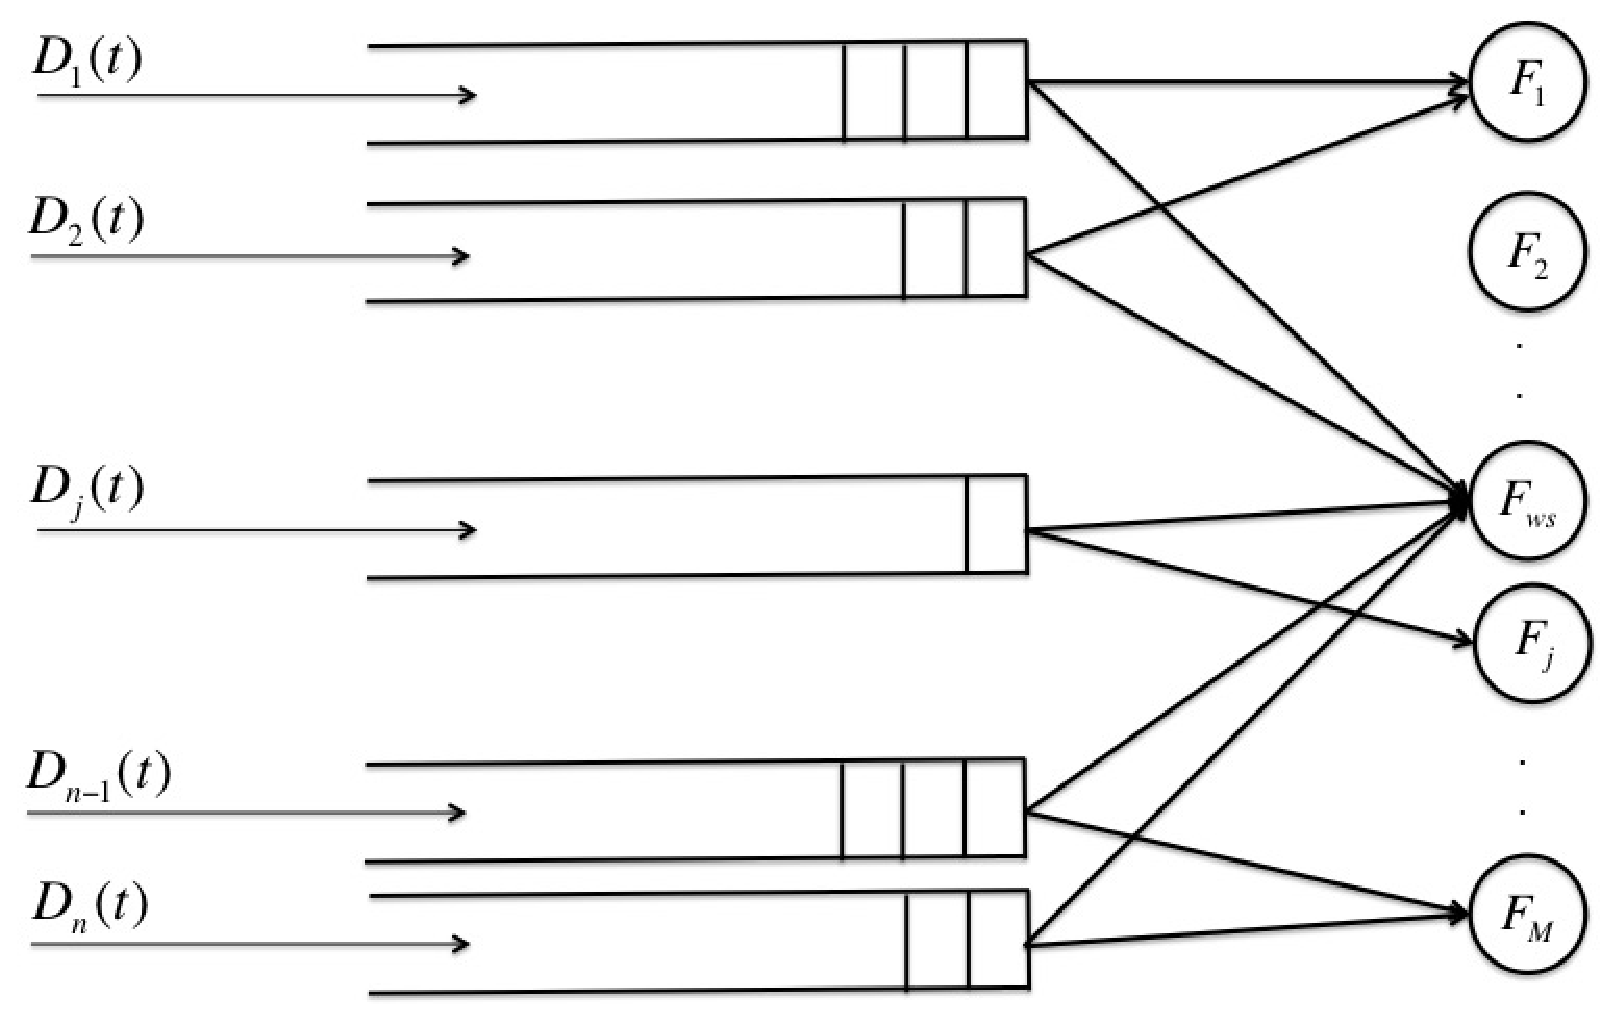
\includegraphics[width=84mm]{figures/flowconfig}
\vspace{-0.1in}
\caption{System Model}
\label{fig:flowconfig}
\vspace{-0.1in}
\end{figure}

The matrix \{$A_{i,j}(t),i\in (F_M+F_w), j\in M$\} denotes the wireless resource association
as shown in Eq.~\ref{eq:associate_def}.
%where $A_{i,j}^b = 1$ denotes user $j$ is scheduled with access point $i$ on channel $b$.
\begin{equation}
\label{eq:associate_def}
 A_{i,j}(t) = \left\{ 
	  \begin{array}{l l}
	    1   &  if\ D_{j\in M},\ is\ associated\ with\ \\
		& radio\ i \in (F_M+F_w) \\
		0 &  Otherwise
			    \end{array} \right.
\end{equation}

To keep the quality of service, the queuing system restricts the expected response time of 
the system $w$ to no more than the tolerance threshold $W$ as shown in Eq.~\ref{eq:timeconstraint}
\begin{equation}
\label{eq:timeconstraint}
E[w]\le W
\end{equation}

% Extreme examples
When the total traffic demand of the users in the system are relatively small, 
the channel capacity of a single white space channel could achieve the quality of 
service in response time for all the users. 
In this scenario, all cell radios could be switched to sleep mode for power saving. 
On the other hand, as the traffic demand increase with the number of users or the demand per 
user, the channel resources need to be increased as the number servers in the queuing system increment 
to meet the user response time tolerance requirements. Thus, in this extreme case, all the radios 
have to keep operating to provide the appropriate quality of service. 
Moreover, when the users are distributed non-uniformly, the long propagated white space channels 
are able to deliver more capacity for the cells with more traffic to balance the system load 
without adding new infrastructure. 
The flexibility of white space channels offers new opportunity for power saving and 
offer load adaptation in network design.
To apply these white space advantages, the question {\it can we save power by exploiting 
the white space capacity with existing cells?} has to be addressed in this system.

In this work, we focus on analyzing the power savings for the heterogeneous 
WhiteCell system. 
To model the power consumption of the system, we sum the power consumption of each operating 
radio in two power consumption categories: standby and transmitting.
We assume the sleeping standby power consumption is negligible as well as the switching power consumption. 
We define $R_i$ represents the radios status in the system, $i\in {F_w,F_M}$. 
The value of $R_i$ denotes the power consumption of the radio for standby and transmitting.
When the radio is in sleeping mode, $R_i = 0$. 
The definition is as represented in Eq.~\ref{eq:radio}.

\begin{equation}
\label{eq:radio}
 R_i(t) = \left\{ 
	  \begin{array}{l l}
	    P_s+P_t\cdot\mu   &  \sum\limits_{j=1}^N A_{i,j}(t) \ge 1\\
		0 &  Otherwise
			    \end{array} \right.
\end{equation}

% Explain the equation
$P_s$ is the standby power consumption of a radio which is a constant value, $P_t$ is the 
unit transmit power consumption of the assigned channel capacity. 
$\mu$ is the allocated channel capacity of the radio.
$R_i(t)$ is the power consumption of the radio during the time slot.

Thus, to reduce the power consumption of the system, it could be 
implemented via minimizing the sum of $R_i$ under the quality of service constraints. 
The objective is to minimize the power consumption of the system is represented in Eq.~\ref{eq:objective}:
\begin{equation}
\label{eq:objective}
R^*(t) = \min{\{\sum\limits_{i=1}^{(F_M+F_w)} R_{i}}(t)\}
%\xi = \min{\{\sum\limits_{t}^{t+T}\sum\limits_{i}^{(F_M+F_w)} R_{i}}(t)\}
\end{equation}
$R^*$ represent the minimum operating power consumption required of the system. 
The allocated resources $\mu$ could be adjusted to approach the minimum power consumption 
in the model. 
According to the queuing quality of service model and power consumption model, 
we further analyze the heterogeneous WhiteCell system and propose our greedy solution.


% Background and problem model
\subsection{Challenges And Analysis}
\label{subsec:challenge}

Prior works model similar multi-channel system as $M/M/m$ queuing system for analyzing.
Other than prior works, this system is not able to be formulated as a $M/M/m$ queuing system due to the 
propagation variation across white space bands and WiFi bands. The users in this system can only be 
served by the white space channels and the WiFi channels assigned in the cell. 
Moreover, we use a measurement based channel estimation other than an on-off channel model in 
this work. 
To design such wireless system, the waiting time constraints have to be satisfied for the quality of service. 
Previous multi-channel works apply $M/M/m$ queuing model for similar system. However, the spectrum 
variation and the white space channel splitting in this system remove the equal service capacity in the system.
Thus, $M/M/m$ queuing system is not directly applicable to get the minimum channel resource which is the
number of servers of the queuing system. 

% User diversity
Also a practical system suffer multi-user diversity.
Multi-user diversity is a form of diversity inherent in a wireless network, provided by 
independent time-varying channels across the different users~\cite{viswanath2002opportunistic}.
% Channel capacity diversity
The user diversity make the channel capacity vary across users. In this system, some WiFi cells may 
have good white space channels while the others may suffer worth white space performance. 
Thus, in-field measurements based channel capacity estimation become an important role in such system.


To answer the design question, we first get the channel capacity from the in-field measurement, then we 
propose a Greedy Server-side Replace (GSR) algorithm to minimize the power consumption and achieve the 
performance constraints.


% User group
The users of the the same WiFi cell are in a heterogeneous queuing system with server of 
WiFi channels and white space channels with service rate $\mu_1,\mu_2,...\mu_{(F_w+1)}$.
The white space channel capacity could be split into multiple WiFi cells, thus, the 
capacity of the white space is usually the minimum channel capacity in a WiFi cell.
The white space channels in a WiFi cell should be less than the WiFi channel or about equal. 
Thus, we apply the transformation model in~\cite{yu2008transformation} to estimate the response 
time $\bar{w}$ which should be less than $W$.
%\label{eq:transformation}
%\mu_{min}=\min{(\mu_1,\mu_2,...\mu_{(F_w+1)})} \\
%\mu_{max}=\max{(\mu_1,\mu_2,...\mu_{(F_w+1)})}//
%k=\frac{\mu_{max}}{\mu_{min}}
%\end{equation}
In this transformation model, the actual arrival rate for one specific server $\lambda_s$ is defined as in 
Eq.~\ref{eq:actarrivalrate}
\begin{equation}
\label{eq:actarrivalrate}
\lambda_s=D/(F_w+1)
\end{equation}

The other parameters are defined in Eq.~\ref{eq:transformation} to~\ref{eq:kvalue}.
\begin{equation}
\label{eq:transformation}
\mu_{min}=\min{(\mu_1,\mu_2,...\mu_{(F_w+1)})} = \bar{\mu}
\end{equation}

\begin{equation}
\mu_{max}=\max{(\mu_1,\mu_2,...\mu_{(F_w+1)})} 
\end{equation}

\begin{equation}
\label{eq:kvalue}
k= \lfloor\frac{\mu_{max}}{\mu_{min}} \rfloor
\end{equation}

When $k=1$, the system could be treated as a homogeneous system. Otherwise,   
$k\ge2$ the average response time of such heterogeneous system could be represented as in Eq.~\ref{eq:heterresponse}\cite{yu2008transformation}:

\begin{equation}
\label{eq:heterresponse}
\bar{w}=\frac{1}{\frac{1}{3}\bar{\mu}(2k+1)-\lambda_s}
\end{equation}

If the traffic could be served only by part of a single white space channel or the WiFi channel, the users in the cell 
converge into a $M/M/1$ queuing. Another scenario is when the traffic occupies two or more channels, the system become 
a $M/M/m$ queuing system. The average response time is calculated as in Eq.~\ref{eq:mm1w} and Eq.~\ref{eq:mmmw}~\cite{gelenbe1998introduction}.
\begin{equation}
\label{eq:mm1w}
\bar{w}=\frac{1}{\mu^+-D}
\end{equation}
$\mu^+$ is the channel capacity of the single server in queuing system.
\begin{equation}
\label{eq:mmmw}
\bar{w} = \frac{1}{\mu^*}(1+\frac{c(m,\rho)}{m(1-\rho)})\approx \frac{1}{\mu^*}\frac{1}{1-\rho^m}
\end{equation}
$\mu^*$ is the channel capacity in the $M/M/m$ queuing system.
$\rho=\frac{\lambda}{m\mu^*}$ is the traffic density, and $c(m,\rho)$ is the Erlang-C formula~\cite{gelenbe1998introduction}.

Through the above analysis, we could calculate the channel capacity need to be spent for certain group of users. 
% Here
% Do I need to consider the rate of the consumption?
To model the power consumption of the system, we assume the power consumption of each operating radio include 
standby and transmitting power.
The operated radios $R_i$ in the system is chosen from the WiFi radios $F_M$ and the white space radios $F_w$. 
If the a radio $R_i$ is chosen, $R_i = 1$, otherwise $R_i = 0$, as shown in Eq.~\ref{eq:radio}
%FIXME need to clarify the \mu, may replace the H with mu

\begin{equation}
\label{eq:radio}
 R_i(t) = \left\{ 
	  \begin{array}{l l}
	    P_s+P_t\cdot\mu   &  \sum\limits_{j=1}^N A_{i,j}(t) \ge 1\\
		0 &  Otherwise
			    \end{array} \right.
\end{equation}


For the carrier, reduce the power consumption is important for cost saving.
Our goal is, during a certain $T$ time slot, to minimize the power consumption as represented in Eq.~\ref{eq:objective}:
\begin{equation}
\label{eq:objective}
R^*(t) = \min{\{\sum\limits_{t=0}^{T}\sum\limits_{i=1}^{(F_M+F_w)} R_{i}}(t)\}
%\xi = \min{\{\sum\limits_{t}^{t+T}\sum\limits_{i}^{(F_M+F_w)} R_{i}}(t)\}
\end{equation}
$R^*$ represent the minimum operating radios power during $T$ time slots required to satisfy the 
users in the system. 

In this model, the less radio we operate in each time slot, the less power consumption will be cost in the system.
To split the white space capacity we propose a Greedy Server-side Replace(GSR) algorithm to approach the minimize 
number of radios operate in the system. The algorithm output the channel resource allocation to satisfy the waiting 
time constraint of the system.


% power consumption extreme
For the power consumption, there are two extremes. When the traffic rate $D$ is low, a white space channel could 
serve all the users in the propagation range. On the other side, when all the WiFi cells have high traffic demand, 
both the WiFi and white space radios have to work for the users. Between the two extremes, when the user traffic 
is medium heavy and the location distribution is non-uniform, the white space channels could adapt these cases.

A white space radio is able to replace a WiFi radio if part of the channel capacity could serve the users in the 
WiFi cell. If each WiFi cell could be served by the least channel resource, the more radios could be turned off. 
The less capacity assigned for the WiFi cells, the less power will be cost for transmission.

\begin{algorithm}[t]
\small
\caption{Greedy Server-side Replace}
\label{algorithm:mape}
\begin{algorithmic}[1]
\REQUIRE  ~~\\
$N$: Users\\
$H_{i,j}^f$: Vector of channel capacity\\
$D$: Traffic Rate\\
$n$: Path Loss Exponent \\
$M$: WiFi Cells
\STATE {Find the WiFi cell with the lowest traffic rate $D$,break the tie with index}
\IF {Check with Eq.~\ref{eq:heterresponse}~\ref{eq:mm1w}~\ref{eq:mmmw} if white space channel satisfy the users, start with the worst/most utilized white space channel}
\STATE Replace the WiFi channel with the white space channel
\STATE Apply half-interval search to find the minimum capacity for the users
\ELSIF {The WiFi channel satisfy the users}
\STATE Keep the WiFi channel and find the minimum capacity for the users
\ELSIF {White space channels available}
\STATE Adding white space resource to the cell
\ELSE 
\STATE Get the response time of the cell with all available resource
\ENDIF
\STATE Update the system information
\STATE Repeat the process for all the cells
\STATE Calculate the power consumption
\ENSURE ~~\\
The power consumption and the maximum response time\\
\end{algorithmic}
\end{algorithm}

The calculation of channel capacity $H$ will be discussed in Section~\ref{sec:experiment}.
The algorithm starts to reduce the standby power then the transmitting power for each server.
%
%
%% Traffic served
%With a schedule $A$, the served traffic flow of a user is the minimize value of the queue with 
%enough channel capacity, or the remaining capacity. The condition $\psi$ as shown in Eq.~\ref{eq:sfcondition}
%\begin{equation}
%\label{eq:sfcondition}
%		\psi =  \sum\limits_{j=1}^N \gamma_j(t) \cdot A_{i,j}(t) 
%		%when \ \sum\limits_{j=1}^N \gamma_j(t) \cdot A_{i,j}(t) > C
%		%	    \end{array} \right.
%\end{equation}
%
%The served traffic flow is represented as in Eq.~\ref{eq:effectiverate}
%\begin{equation}
%\label{eq:effectiverate}
% \gamma_j(t) = \left\{ 
%	  \begin{array}{l l}
%	     \min\limits_{j\in N}(Q_j(t),\sum\limits_{i=1}^{F_M+F_w} A_{i,j}(t) \cdot H_{i,j}(t)) & \psi \le C    \\ 
%		 0 & \psi > C
%			    \end{array} \right.
%\end{equation}
%
%
%
%% The length of the queue
%The new arrival traffic demand $D_i(t)$ can not be served at the current time slot $t$.
%The individual queues $Q_j(t),j\in N$ at the end of the time slot $t$ is represented as Eq.~\ref{eq:userqueue}:
%\begin{equation}
%\label{eq:userqueue}
%%Q_j(t) = Q_j(t-1)+D_j(t)-\min{\{\sum\limits_{i=1}^{(F_m+F_w)} H_{i,j}(t)\cdot A_{i,j}(t),Q_j(t-1)}\}
%Q_j(t) = Q_j(t-1)+D_j(t)- \gamma_j(t)
%\end{equation}
%
%
%
%% Here D is preknow in T slots and discuss the T constraints
%In this system, the channel capacity $H_{i,j}^f(t)$ is from the SNR according to 
%Friis model and in-field measurements. We consider discrete time with a suitably 
%chosen small time unit. %One user can only associate 
%%with a single channel during a time slot to avoid heavy interference. 
%Users scheduled with the same channel will share the time unit through time division inside 
%the time slot. 
%
%% Constraints
%
%
%% Discuss the feasibility of buffer
%The minimize number of operating radios has to fulfill the maximize capacity of each user greater than 
%the remaining buffer and the new coming data as shown in Eq.~\ref{eq:capacity}
%\begin{equation}
%\label{eq:capacity}
%\sum\limits_{j=1}^{F_m+F_b}H_{ij}(T)\ge Q_i(T) ,\ i\in N
%\end{equation}
%Otherwise the buffer will be overflow, and there is no feasible solution of the system.




% Linear is not good enough complexity unsure channel state


% Greedy algorithm








% Channel state estimation








% Reduce the radio/server/channel resource



% New section feasibility, and Max flow formulation

%The model could be formulated as a {\it Max-Flow} problem~\cite{networkoptimization}. The question is 
%looking for a feasible flow $\Gamma$ under the constraints of channel capacity $H$ and traffic demand $D$. 
%The lower bound of flow is $0$, the upper bound of a single flow from the accss point $i$ to user $j$ is 
%the measurements based $H_{i,j}^b$.
%Thus, $\gamma_j \le \sum\limits_{i\in M} \sum\limits_{b \in B} H_{i,j}^b\cdot A_{i,j}^b$. The max-flow model 
%of the problem is feasible. 











% Greedy algorithm








% Channel state estimation








% Reduce the radio/server/channel resource



% New section feasibility, and Max flow formulation

%The model could be formulated as a {\it Max-Flow} problem~\cite{networkoptimization}. The question is 
%looking for a feasible flow $\Gamma$ under the constraints of channel capacity $H$ and traffic demand $D$. 
%The lower bound of flow is $0$, the upper bound of a single flow from the accss point $i$ to user $j$ is 
%the measurements based $H_{i,j}^b$.
%Thus, $\gamma_j \le \sum\limits_{i\in M} \sum\limits_{b \in B} H_{i,j}^b\cdot A_{i,j}^b$. The max-flow model 
%of the problem is feasible. 


\section{Experiment and Analysis}
\label{sec:experiment}

In this section, we introduce the measurements experiments setup and 
evaluate the process of probabilistic forecasting of channel state.
Based on the probabilistic forecasting result, we perform numeric
simulation of the Bayesian Beam Schedule. We further compare the 
performance of BBS to the equal time schedule and maximum channel 
capacity schedule and show the gain of the BBS with analysis.


% Subsec Experiment design
\subsection{Experiment Design}
\label{subsec:experimentdesign}

The BBS is a measurements driven method, espicelly for the probabilistic forecasting
of the channel states of each client. We perform experiments with an Android application, 
WiEye worldwide measurements. And also we perform small scale local measurements in typical downtown,
urban, neighborhood and campus area.

% Wieye
The application for the data collection is currently available for download and usage via the Google 
Android Marketunder the name WiEye. Users are able to view all Wi-Fi access points that are within range 
oftheir cellular device in both graphical and tabular form. All datacollection is done in the background, 
either continuously while theuser is running the application or periodically if the user has optedin to 
background data collection to assist our study. Our data collection has been approved by the Southern 
Methodist UniversityInstitutional Review Board, a human subjects research committee, ensuring that all 
ethical precautions have been taken in collectingdata from the users of our application.

Through this piece of data, we investigate the large scale beam schedule through BBS in a city.
FIXME

% Local Measurements 
We employ a Linux-based 802.11 testbed, which includes aGateworks 2358 board with Ubiquiti XR radios 
(XR9 at 900MHz, XR2 at 2.4 GHz, XR5 at 5.2 GHz) and a DoodleLabsDL475 radio at 450 MHz. We develop shell 
scripts whichutilize tcpdump to enable the testbed to work as a sniffer,recording all 802.11 packets. 
However, since the Gateworksplatform only updates its estimate of received signal strengthupon the 
reception of a new packet (and not all relevantchannel activity is 802.11 based), we employ a spectrumanalyzer 
to form a notion of inter-network interference withfiner granularity. Hence, we also use a Rohde \& Schwarz FSH 8 
portable spectrum works from 100 KHz to 8 GHz. Theportable spectrum analyzer is controlled by a Python 
script on a laptop to measure the received signal strength.

Through the local measurements, we explore the application in small scale which the measurements has more 
correlation with each other.
FIXME

\subsection{Numerical Simulation}
\label{subsec:result}

% Network setup, area, beams,traffic, payoff parameters
In the part, we set up a measurements driven simulation to evaluate the performance of the BBS framework.
And we further compare the performance with the non beam forming access, equal time schedule, and the post 
upper bound of beam schedule. In the non beam forming access, we omit the RTS/CTS time cost in the simulation.
Equal time schedule is to schedule the beam equally to all the clients in the served area. In the post upper
bound beam schedule, we already know the best channel state, in such situation, we can update the beam schedule
with the best options.
% Area Here
We choose 3 pieces of measurements data in the simulations. One from the measurements from a public park near
our campus, one from the WiEye data in a major city in US, the last one set is from the WiEye data in an 
urban area. Dense area with more traffic demands is more applicable for beam forming technology.

% Setup
In the first public scenario, we looked up the access points from Google(FIXME) and select the clients from the 
measurements we got from the area.


From the measurements, we analysis the activities across time and output the variation of time domain.
Large scale application

Small scale application

% Measurements and probabilistic forecasting




% Bayesian beam schedule




% Compare with other method










\section{Related Work}
\label{sec:related}


% White Space
Since white space bands were free for wireless communication, many efforts have been 
put in the area for the application of white space bands.~\cite{fccwhitespace} 
In~\cite{bahl2009white}. the author considered a cognitive method to avoid collision 
between white space communication and TV broadcasting. 
Many works increasing the convenience of using white space databases have been published 
(e.g., Microsoft's White Space Database~\cite{msdatabase}).
Google has even visualized the licensed white space channels 
in US cities with an API for research and commercial use~\cite{googledatabase}.
Previous work discussed the point to point communication with white space bands~\cite{cui2013leveraging}, 
and the wireless network deployment with plenty white space channels~\cite{pcuiwinmee}.
However, many of the major cities in the US do not have plenty white space channels, such as 
most area of Austin, TX has only one white space channel. As far as we know, there is no work 
discuss these scenarios.


%  Multi-channel
Applying white space in wireless network is similar to the previous multi-channel works other the 
propagation variation. In~\cite{bodas2012low} a multi-channel system is formulated as a queuing 
system and Server Side Greedy algorithm is proposed to optimize the throughput with low complexity. 
In~\cite{ji2013performance}, Delay-based Queue-Side-Greedy algorithm is proposed with low complexity 
for optimal throughput and near-optimal delay.~\cite{liu2014energy} develop a multi-objective optimization 
framework to minimal energy consumption in a multi-channel multi-radio system. 
However, these works do not address minimizing the resource for certain quality of service and assume an 
on-off channel model.

% Need to modify
Previous work studied the multi user setting with a single channel~\cite{tan2010distributed}. 
Spectral diversity is isolated for a single user in~\cite{shu2009throughput}. In~\cite{liu2013stay}, 
multi-user dynamic channel access is proposed jointly consider the temporal and spectral diversity in a multichannel model. However, 
none of these works address the channel association problem in multiband scenario.
Previous work~\cite{pcuiwinmee} studied the 
white space application in access network deployment with spectral diversity. However, these works 
fails to leverage the white space frequency in multi-user diversity in both spectral and temporal scenarios.

%% Multithread
% On-off channel
Previous works in real time systems put many efforts to minimize the resources, such as processors~\cite{nelissen2012techniques}.
In~\cite{li2014analysis}, the author proves the capacity augmentation bounds for schedulers of parallel tasks. 
However, these works assume the parallel tasks have uniform servers. 
Previous work~\cite{chen2011feasibility} investigate the white space in a queuing system without considering the 
heterogeneous topology.
In contrast, we study the performance of a heterogeneous network with both white space channels 
and WiFi channels in channel utilization. 

% gan2014multiple

% weighted sum/less info





\section{Conclusion}
\label{sec:conclusion}
In this paper
% Future work



\bibliographystyle{IEEEtran}

\bibliography{whitecell}

\end{document}
